\documentclass{ximera}

\author{Bart Snapp}

\newcommand{\RR}{\mathbb R}
\renewcommand{\d}{\,d}
\newcommand{\dd}[2][]{\frac{d #1}{d #2}}
\renewcommand{\l}{\ell}
\newcommand{\ddx}{\frac{d}{dx}}
\newcommand{\dfn}{\textbf}
\newcommand{\eval}[1]{\bigg[ #1 \bigg]}


\outcome{Use Green's Theorem as a planimeter.}

\title[Dig-In:]{Green's Theorem as a planimeter}

\begin{document}
\begin{abstract}
  A planimeter computes the area of a region by tracing the boundary.
\end{abstract}
\maketitle

Green's Theorem may seem rather abstract, but as we will see, it is a
fantastic tool for computing the areas of arbitrary bounded
regions. In particular, Green's Theorem is a theoretical
\link[planimeter]{http://en.wikipedia.org/wiki/Planimeter}. A
\dfn{planimeter} is a ``device'' used for measuring the area of a
region. Ideally, one would ``trace'' the border of a region, and the
planimeter would tell you the area of the region.


\section{How is Green's Theorem a planimeter?}

Recall Green's Theorem:
\begin{theorem}[Green's Theorem]\index{Green's Theorem}
  If the components of $\vec{F}:\R^2\to\R^2$ have continuous partial
  derivatives and $C$ is a boundary of a closed region $R$ and
  $\vec{p}(t)$ parameterizes $C$ in a counterclockwise direction with
  the interior on the left, then
  \[
  \iint_R \curl\vec{F}\d A = \oint_C \vec{F}\dotp\d\vec{p} 
  \]
\end{theorem}

Given a vector field $\vec{F}:\R^2\to\R^2$, if $\curl\vec{F} = 1$,
then the left-hand side of the conclusion of Green's Theorem gives the
area of the region $R$:
\[
\iint_R \curl\vec{F}\d A = \iint_R \d A
\]

So now the question becomes, which vector fields have $\curl\vec{F} =
1$? Here are three basic candidates:
\begin{itemize}
\item $\vec{F}(x,y) = \vector{0,x}$
\item $\vec{F}(x,y) = \vector{-y,0}$
\item $\vec{F}(x,y) = \vector{-y/2,x/2}$
\end{itemize}
\begin{question}
  The key idea that connects the three vector fields above is:
  \begin{selectAll}
    \choice[correct]{Their curl is $1$.}
    \choice{They are conservative fields.}
    \choice{They are gradient fields.}
    \choice[correct]{When used in combination with Green's Theorem, they help compute area.}
  \end{selectAll}
\end{question}

Once we have a vector field whose curl is $1$, we may then apply
Green's Theorem to use a line integral to compute the area.

\begin{warning}
  You must parameterize $C$ with $\vec{p}(t)$ for $a\le t\le b$ such that:
  \begin{itemize}
    \item $C$ is drawn in a counterclockwise direction.
    \item $C$ is drawn exactly once.
    \item The interior of $R$ is to the left of the direction of
      $\vec{p}'(t)$.
  \end{itemize}
\end{warning}




\section{Computing areas with Green's Theorem}

Now let's do some examples.

\begin{example}
  Compute the area of the trapezoid below using Green's Theorem.
  \begin{image}
    \begin{tikzpicture}
      \begin{axis}%
        [
	  ymin=-.5,ymax=2.5,
	  xmin=-.5,xmax=4.5,
          axis lines =middle, xlabel=$x$, ylabel=$y$,
          every axis y label/.style={at=(current axis.above origin),anchor=south},
          every axis x label/.style={at=(current axis.right of origin),anchor=west},
          grid=both,
          grid style={dashed, gridColor},
          % xtick={-2,...,4},
          % ytick={-3,...,3},
	]
        \addplot[penColor,ultra thick] coordinates{
            (0,0) (1,2) (3,2) (4,0) (0,0) (1,2)
        };
        
      \end{axis}
    \end{tikzpicture}
  \end{image}
  \begin{explanation}
    In this case, set $\vec{F}(x,y) = \vector{0,x}$. Since $\curl\vec{F} =
    1$, Green's Theorem says:
    \[
    \iint_R \d A  = \oint_C \vector{0,x}\dotp\d\vec{p}
    \]
    We need to parameterize our paths in a counterclockwise
    direction. We'll break it into four line segments each parameterized
    as $t$ runs from $0$ to $1$:
    \begin{image}
      \begin{tikzpicture}
        \begin{axis}%
          [
	  ymin=-.5,ymax=2.5,
	  xmin=-.5,xmax=4.5,
          axis lines =middle, xlabel=$x$, ylabel=$y$,
          every axis y label/.style={at=(current axis.above origin),anchor=south},
          every axis x label/.style={at=(current axis.right of origin),anchor=west},
          grid=both,
          grid style={dashed, gridColor},
         % xtick={-2,...,4},
         % ytick={-3,...,3},
	]
        \addplot[penColor,ultra thick] coordinates{
            (0,0) (1,2) 
        };
        \addplot[penColor,->,ultra thick] coordinates{
            (1,2) (.5,1) 
        };
        
        \addplot[penColor2,ultra thick] coordinates{
            (1,2) (3,2) 
        };
        \addplot[penColor2,ultra thick,->] coordinates{
            (3,2) (2,2) 
        };
        
        \addplot[penColor4,ultra thick] coordinates{
            (3,2) (4,0) 
        };
        \addplot[penColor4,ultra thick,->] coordinates{
            (4,0) (3.5,1) 
        };
        
        \addplot[penColor5,ultra thick] coordinates{
            (4,0) (0,0) 
        };
        \addplot[penColor5,ultra thick,->] coordinates{
            (0,0) (2,0) 
        };
        
        \node[above,penColor5] at (axis cs: 2,0) {$\vecl_1$};
        \node[penColor4] at (axis cs: 3.2,1) {$\vecl_2$};
        \node[below,penColor2] at (axis cs: 2,2) {$\vecl_3$};
        \node[penColor] at (axis cs: .8,1) {$\vecl_4$};

        \end{axis}
      \end{tikzpicture}    
    \end{image}
    where:
    \begin{align*}
      \vecl_1(t) &= \vector{4t,\answer[given]{0}}\\
      \vecl_2(t) &= \vector{\answer[given]{4-t},2t}\\
      \vecl_3(t) &= \vector{3-2t,\answer[given]{2}}\\
      \vecl_4(t) &= \vector{\answer[given]{1-t},2-2t}
    \end{align*}
    and each draws the line as $t$ runs from $0$ to $1$.  Write:
    \begin{align*}
      \oint_C \vec{F}\dotp\d\vec{p} = \int_0^1 &\vec{F}(\vecl_1(t))\dotp \vecl_1'(t) \d t
    + \int_0^1 \vec{F}(\vecl_2(t))\dotp \vecl_2'(t) \d t\\
    &+ \int_0^1 \vec{F}(\vecl_3(t))\dotp \vecl_3'(t) \d t
    + \int_0^1 \vec{F}(\vecl_4(t))\dotp \vecl_4'(t) \d t
    \end{align*}
    For each of the integrands above, say $\vecl(t) =
    \vector{x(t),y(t)}$, we will write
    \[
    \vec{F}(\vecl(t))\dotp \vecl'(t) = \vector{0,x(t)} \dotp \vector{x'(t),y'(t)}
    \]
    and combine them into a single integral. Write with me
    \begin{align*}
      \oint_C \vec{F}\dotp\d\vec{p} &= \int_0^1 \left(\answer[given]{2(4-t) -2(1-t)} \right)\d t\\
      &= \eval{\answer[given]{6t}}_0^1\\
      &=\answer[given]{6}. 
    \end{align*}
    So the this is the area of the trapezoid.
  \end{explanation}
\end{example}

\begin{example}
  Compute the area of the ellipse
  \[
  \frac{x^2}{a^2} + \frac{y^2}{b^2} = 1
  \]
  using Green's Theorem.
  \begin{explanation}
    To start, we'll set $\vec{F}(x,y) = \vector{-y/2,x/2}$. Since
    $\curl\vec{F} = 1$, Green's Theorem says:
    \[
    \iint_R \d A  = \oint_C \vector{-y/2,x/2}\dotp\d\vec{p}
    \]
    We can parameterize the boundary of the ellipse with
    \begin{align*}
      x(t) &= a \cos(t)\\
      y(t) &= b \sin(t)
    \end{align*}
    for $0\le t<2\pi$. Write with me
    \begin{align*}
      \iint_R \d A &= \oint_C \vector{-y/2,x/2}\dotp\vector{x'(t),y'(t)}\d t\\
      &= \int_0^{2\pi} \vector{\answer[given]{-b\sin(t)/2},\answer[given]{a\cos(t)/2}}\dotp\vector{\answer[given]{-a\sin(t)},\answer[given]{b\cos(t)}}\d t\\
      &= \int_0^{2\pi} (1/2)\left(ab\sin^2(t) + ab\cos^2(t)\right) \d t\\
      &= \int_0^{2\pi} (1/2)ab \d t\\
      &= \answer[given]{\pi ab}. 
    \end{align*}
    Done. Green's Theorem for the win!
  \end{explanation}
\end{example}

Finally, what do you do if you have a very strangely shaped curve? You approximate it with a polygonal curve. Check out next example.

\begin{example}
  Compute the area of the polygonal region below using Green's Theorem.
  \begin{image}
    \begin{tikzpicture}
      \begin{axis}%
        [
	  ymin=-3.2,ymax=3.2,
	  xmin=-3.2,xmax=4.2,
          axis lines =middle, xlabel=$x$, ylabel=$y$,
          every axis y label/.style={at=(current axis.above origin),anchor=south},
          every axis x label/.style={at=(current axis.right of origin),anchor=west},
          grid=both,
          grid style={dashed, gridColor},
          xtick={-3,...,4},
          ytick={-3,...,3},
	]
        \addplot[penColor,ultra thick] coordinates{
          (1,-1) (3,1) (0,1) (-1,3) (-2,-1) (1,-3)
          (1,-1) (3,1)
        };
        
      \end{axis}
    \end{tikzpicture}
  \end{image}
  \begin{explanation}
    In this case, set $\vec{F}(x,y) = \vector{0,x}$. Now we'll break this curve
    into six line segments that draw this curve in a counterclockwise
    fashion as a parameter $t$ runs from $0$ to $1$.
    \begin{image}
    \begin{tikzpicture}
      \begin{axis}%
        [
	  ymin=-3.2,ymax=3.2,
	  xmin=-3.2,xmax=4.2,
          axis lines =middle, xlabel=$x$, ylabel=$y$,
          every axis y label/.style={at=(current axis.above origin),anchor=south},
          every axis x label/.style={at=(current axis.right of origin),anchor=west},
          grid=both,
          grid style={dashed, gridColor},
          xtick={-3,...,4},
          ytick={-3,...,3},
	]
        \addplot[penColor,ultra thick] coordinates{
          (1,-1) (3,1) 
        };
        \addplot[penColor,ultra thick,->] coordinates{
          (1,-1) (2,0) 
        };
        
        \addplot[penColor2,ultra thick] coordinates{
          (3,1) (0,1) 
        };
        \addplot[penColor2,ultra thick,->] coordinates{
          (3,1) (1.5,1) 
        };
        
        \addplot[penColor3,ultra thick] coordinates{
          (0,1) (-1,3) 
        };
        \addplot[penColor3,ultra thick,->] coordinates{
          (0,1) (-.5,2) 
        };
        
        \addplot[penColor4,ultra thick] coordinates{
          (-1,3) (-2,-1) 
        };
        \addplot[penColor4,ultra thick,->] coordinates{
          (-1,3) (-1.5,1) 
        };
        
        \addplot[penColor5,ultra thick] coordinates{
          (-2,-1) (1,-3)
        };
        \addplot[penColor5,ultra thick,->] coordinates{
          (-2,-1) (-.5,-2)
        };
        
        \addplot[yellow!70!black,ultra thick] coordinates{
          (1,-3) (1,-1)
        };
        \addplot[yellow!70!black,ultra thick,->] coordinates{
          (1,-3) (1,-2)
        };
        \node[above left,penColor] at (axis cs: 2,0) {$\vecl_1$};
        \node[penColor2,above] at (axis cs: 1.5,1) {$\vecl_2$};
        \node[below left,penColor3] at (axis cs: -.5,2) {$\vecl_3$};
        \node[left,penColor4] at (axis cs: -1.5,1) {$\vecl_4$};
        \node[below,penColor5] at (axis cs: -.5,-2) {$\vecl_5$};
        \node[right,penColor6] at (axis cs: 1,-2) {$\vecl_6$};       
        
      \end{axis}
    \end{tikzpicture}
    \end{image}
    where:
    \begin{align*}
      \vecl_1(t) &= \vector{1+2t,\answer[given]{-1+2t}}\\
      \vecl_2(t) &= \vector{\answer[given]{3-3t},1}\\
      \vecl_3(t) &= \vector{-t,\answer[given]{1+2t}}\\
      \vecl_4(t) &= \vector{-1-t,\answer[given]{3-4t}}\\
      \vecl_5(t) &= \vector{\answer[given]{-2+3t},-1-2t}\\
      \vecl_6(t) &= \vector{1,\answer[given]{-3+2t}}
    \end{align*}
    and each draws the line as $t$ runs from $0$ to $1$.  Write:
    \begin{align*}
      \oint_C \vec{F}\dotp\d\vec{p} =
      &\int_0^1 \vec{F}(\vecl_1(t))\dotp \vecl_1'(t) \d t\\
      &+ \int_0^1 \vec{F}(\vecl_2(t))\dotp \vecl_2'(t) \d t\\
      &+ \int_0^1 \vec{F}(\vecl_3(t))\dotp \vecl_3'(t) \d t\\
      &+ \int_0^1 \vec{F}(\vecl_4(t))\dotp \vecl_4'(t) \d t\\
      &+ \int_0^1 \vec{F}(\vecl_5(t))\dotp \vecl_5'(t) \d t\\
      &+ \int_0^1 \vec{F}(\vecl_6(t))\dotp \vecl_6'(t) \d t
    \end{align*}
    For each of the integrands above, say $\vecl(t) =
    \vector{x(t),y(t)}$, we will write
    \[
    \vec{F}(\vecl(t))\dotp \vecl'(t) = \vector{0,x(t)} \dotp \vector{x'(t),y'(t)}
    \]
    and combine them into a single integral. Write with me
    \begin{align*}
      \oint_C \vec{F}\dotp\d\vec{p} &= \int_0^1 \left(\answer[given]{12} \right)\d t\\
      &= \eval{\answer[given]{12t}}_0^1\\
      &=\answer[given]{12}. 
    \end{align*}
    So the this is the area of the region.
  \end{explanation}
\end{example}

Green's Theorem gives a fairly easy method for computing any the area
of any polygonal region. Any region with a ``smooth'' border can be approximated by a polygonal region. The upshot? Green's Theorem is a powerful tool for computing area.



\section{The shoelace algorithm}\index{shoelace algorithm}

Green's Theorem can also be used to derive a simple (yet powerful!)
algorithm (often called the ``shoelace'' algorithm) for computing
areas. Here's the idea: Suppose you have a two-dimensional polygon,
where the vertices are identified by their $(x,y)$-coordinates:
\begin{image}
  \begin{tikzpicture}
    \begin{axis}%
      [
	ymin=0,ymax=12,
	xmin=0,xmax=16,
        axis lines=none,
        clip=false
      ]
      
      \addplot[penColor,ultra thick] coordinates{
        (6,11) (4,10) (2,6) (3,3) (8,2) (14,5) (9,6) (14,8) (12,10) (8,7)
      };

       \addplot[penColor!50!white,dashed,ultra thick] coordinates{
        (6,11) (8,7)
       };
      
       \addplot[color=penColor,fill=penColor,only marks,mark=*] coordinates{(6,11)};  %% closed hole
       \addplot[color=penColor,fill=penColor,only marks,mark=*] coordinates{(4,10)};  %% closed hole
       \addplot[color=penColor,fill=penColor,only marks,mark=*] coordinates{(2,6)};  %% closed hole
       \addplot[color=penColor,fill=penColor,only marks,mark=*] coordinates{(3,3)};  %% closed hole
       \addplot[color=penColor,fill=penColor,only marks,mark=*] coordinates{(8,2)};  %% closed hole
       \addplot[color=penColor,fill=penColor,only marks,mark=*] coordinates{(14,5)};  %% closed hole
       \addplot[color=penColor,fill=penColor,only marks,mark=*] coordinates{(9,6)};  %% closed hole
       \addplot[color=penColor,fill=penColor,only marks,mark=*] coordinates{(14,8)};  %% closed hole
       \addplot[color=penColor,fill=penColor,only marks,mark=*] coordinates{(12,10)};  %% closed hole
       \addplot[color=penColor,fill=penColor,only marks,mark=*] coordinates{(8,7)};  %% closed hole
       
       \node[penColor, left] at (axis cs: 4,10) {$(x_1,y_1)$};
       \node[penColor, left] at (axis cs: 2, 6) {$(x_2,y_2)$};
       \node[penColor,below left] at (axis cs: 3, 3) {$(x_3,y_3)$};
       \node[penColor,below] at (axis cs: 8, 2) {$(x_4,y_4)$};
       \node[penColor,right] at (axis cs:14, 5) {$(x_5,y_5)$};
       \node[penColor, left] at (axis cs: 9, 6) {$(x_6,y_6)$};
       \node[penColor,right] at (axis cs:14, 8) {$(x_7,y_7)$};
       \node[penColor,right] at (axis cs:12,10) {$(x_8,y_8)$};
       \node[penColor, left] at (axis cs: 8, 7) {$(x_9,y_9)$};
       \node[penColor,right] at (axis cs: 6,11) {$(x_n,y_n)$};
    \end{axis}
  \end{tikzpicture}
\end{image}
Here we see a polygon with $n$ vertices, and the ``dashed-line''
means that there could be more to this polygon than ``meets the
eye.'' So to compute the area, here is a neat trick. Write all of
the coordinates in a column, writing the starting coordinate
\textit{twice}, both at the beginning and at the end:

\begin{image}[.5in]
  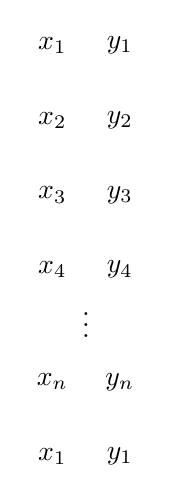
\begin{tikzpicture}
    \begin{axis}%
      [
	ymin=0,ymax=12,
	xmin=0,xmax=16,
        axis lines=none,
        clip=false
      ]      
      \node at (axis cs:0,12) {$x_1$};
      \node at (axis cs:2,12) {$y_1$};
      
      \node at (axis cs:0,10) {$x_2$};
      \node at (axis cs:2,10) {$y_2$};
      
      \node at (axis cs:0, 8) {$x_3$};
      \node at (axis cs:2, 8) {$y_3$};
      
      \node at (axis cs:0, 6) {$x_4$};
      \node at (axis cs:2, 6) {$y_4$};

      \node at (axis cs:1, 4.75) {$\vdots$};
      
      \node at (axis cs:0, 3) {$x_n$};
      \node at (axis cs:2, 3) {$y_n$};
      
      \node at (axis cs:0, 1) {$x_1$};
      \node at (axis cs:2, 1) {$y_1$};
    \end{axis}
  \end{tikzpicture}
\end{image}

Now multiply entries of the columns diagonally down from the left to the right and add them together

\begin{image}[.5in]
  \begin{tikzpicture}
    \begin{axis}%
      [
	ymin=0,ymax=12,
	xmin=0,xmax=16,
        axis lines=none,
        clip=false
      ]      
      \node at (axis cs:0,12) {$x_1$};
      \node at (axis cs:2,12) {$y_1$};

      \addplot[->,ultra thick,penColor,shorten >=0.2cm,shorten <=.2cm,] coordinates{(0,12) (2,10)};
      
      \node at (axis cs:0,10) {$x_2$};
      \node at (axis cs:2,10) {$y_2$};

      \addplot[->,ultra thick,penColor,shorten >=0.2cm,shorten <=.2cm,] coordinates{(0,10) (2,8)};
      
      \node at (axis cs:0, 8) {$x_3$};
      \node at (axis cs:2, 8) {$y_3$};

      \addplot[->,ultra thick,penColor,shorten >=0.2cm,shorten <=.2cm,] coordinates{(0,8) (2,6)};
      
      \node at (axis cs:0, 6) {$x_4$};
      \node at (axis cs:2, 6) {$y_4$};

      %\addplot[->,ultra thick,penColor,shorten >=0.2cm,shorten <=.2cm,] coordinates{(0,6) (2,4)};

      \node at (axis cs:1, 4.75) {$\vdots$};

      %\addplot[->,ultra thick,penColor,shorten >=0.2cm,shorten <=.2cm,] coordinates{(0,5) (2,3)};
      
      \node at (axis cs:0, 3) {$x_n$};
      \node at (axis cs:2, 3) {$y_n$};

      \addplot[->,ultra thick,penColor,shorten >=0.2cm,shorten <=.2cm,] coordinates{(0,3) (2,1)};
      
      \node at (axis cs:0, 1) {$x_1$};
      \node at (axis cs:2, 1) {$y_1$};
    \end{axis}
  \end{tikzpicture}
\end{image}
to obtain:
\[
x_1y_2 + x_2y_3 + x_3y_4 + \dots + x_ny_1
\]
Now, multiply entries of the columns diagonally down from the left to
the right and subtract them from our previous sum
\begin{image}[.5in]
  \begin{tikzpicture}
    \begin{axis}%
      [
	ymin=0,ymax=12,
	xmin=0,xmax=16,
        axis lines=none,
        clip=false
      ]      
      \node at (axis cs:0,12) {$x_1$};
      \node at (axis cs:2,12) {$y_1$};

      \addplot[->,ultra thick,penColor!50!white,shorten >=0.2cm,shorten <=.2cm,] coordinates{(0,12) (2,10)};
      \addplot[->,ultra thick,penColor2,shorten >=0.2cm,shorten <=.2cm,] coordinates{(2,12) (0,10)};
      
      \node at (axis cs:0,10) {$x_2$};
      \node at (axis cs:2,10) {$y_2$};

      \addplot[->,ultra thick,penColor!50!white,shorten >=0.2cm,shorten <=.2cm,] coordinates{(0,10) (2,8)};
      \addplot[->,ultra thick,penColor2,shorten >=0.2cm,shorten <=.2cm,] coordinates{(2,10) (0,8)};
      
      \node at (axis cs:0, 8) {$x_3$};
      \node at (axis cs:2, 8) {$y_3$};

      \addplot[->,ultra thick,penColor!50!white,shorten >=0.2cm,shorten <=.2cm,] coordinates{(0,8) (2,6)};
      \addplot[->,ultra thick,penColor2,shorten >=0.2cm,shorten <=.2cm,] coordinates{(2,8) (0,6)};
      
      \node at (axis cs:0, 6) {$x_4$};
      \node at (axis cs:2, 6) {$y_4$};

      %\addplot[->,ultra thick,penColor!50!white,shorten >=0.2cm,shorten <=.2cm,] coordinates{(0,6) (2,4)};

      \node at (axis cs:1, 4.75) {$\vdots$};

      %\addplot[->,ultra thick,penColor!50!white,shorten >=0.2cm,shorten <=.2cm,] coordinates{(0,5) (2,3)};
      
      \node at (axis cs:0, 3) {$x_n$};
      \node at (axis cs:2, 3) {$y_n$};

      \addplot[->,ultra thick,penColor!50!white,shorten >=0.2cm,shorten <=.2cm,] coordinates{(0,3) (2,1)};
      \addplot[->,ultra thick,penColor2,shorten >=0.2cm,shorten <=.2cm,] coordinates{(2,3) (0,1)};
      
      \node at (axis cs:0, 1) {$x_1$};
      \node at (axis cs:2, 1) {$y_1$};
    \end{axis}
  \end{tikzpicture}
\end{image}
to obtain:
\begin{align*}
  S=x_1y_2 &+ x_2y_3 + x_3y_4 + \dots + x_ny_1 \\
  &-x_2y_1 - x_3y_2 - x_4y_3 - \dots - x_1y_n
\end{align*}
The area of the polygon in question will be:
\[
A = \frac{|S|}{2}
\]
The algorithm is called the ``shoelace'' algorithm because of the
crisscrossing pattern you see above.

\begin{question}
  Compute the area of the following polygon:
  \begin{image}
    \begin{tikzpicture}
      \begin{axis}%
        [
	  xmin=-8,xmax=8,
          ymin=-8,ymax=8,
          xlabel=$x$,ylabel=$y$,
          axis lines=center,
          every axis y label/.style={at=(current axis.above origin),anchor=south},
          every axis x label/.style={at=(current axis.right of origin),anchor=west},
          clip=false,
	  grid =major,
          xtick={-8,-7,...,8},
          ytick={-8,-7,...,8},
	]
        \addplot[line join =bevel,penColor,ultra thick] coordinates{
          (5,5)   (1,2)   (0,7)  (-1,2) (-5,5) (-2,1) (-7,-1)
          (-2,-1) (-4,-6) (0,-2) (4,-6) (2,-1) (7,-1) (2,1) (5,5) (1,2)};
      \end{axis}
    \end{tikzpicture}
  \end{image}
  \begin{prompt}
    The area is $\answer{47}$ square units.
  \end{prompt}
\end{question}

\subsection{Why does the shoelace algorithm work?}

Now we are going explain why the shoelace algorithm works via Green's
Theorem. The restrained young mathematician may protest that we are
using a ``crane to crush a fly,'' but whatever. We \textit{like}
Green's Theorem.

\begin{algorithm}[Shoelace]\index{shoelace algorithm}
  Given a polygon $P$ with vertices at
  \[
  (x_1,y_1),(x_2,y_2),\dots,(x_n,y_n)
  \]
  we may compute the area of the polygonal region $R$ by setting
  $(x_{n+1},y_{n+1} = (x_1,y_1)$ and computing:
  \[
  \text{area} = \frac{1}{2}\left|\sum_{i=1}^n \left(x_iy_{i+1} - x_{i+1}y_i\right)\right|
  \]
  \begin{explanation}
    To start, recall that if $\vec{F} = \vector{0,x}$, then
    $\curl\vec{F}(x,y) = 1$. Hence Green's Theorem states:
    \[
    \iint_R \d A = \oint_P x\d y
    \]
    This means we can compute the area of the region $R$, by
    evaluating the line integral on the right along the polygonal
    boundary $P$. Since we're supposing that the vertices of the
    polygon are
    \[
    (x_1,y_1),(x_2,y_2),\dots,(x_n,y_n)
    \]
    $P$ can be broken into $n$ edges, (if a polygon has $n$ vertices,
    it has $n$ edges). We can parameterize each edge as
    \begin{align*}
      E_1 &: \vector{x_1,y_1} + t \vector{x_2-x_1,y_2-y_1}\\
      E_2 &: \vector{x_2,y_2} + t \vector{x_3-x_2,y_3-y_2}\\
      E_3 &: \vector{x_3,y_3} + t \vector{x_4-x_3,y_4-y_3}\\
      &\vdots\\
      E_n &: \vector{x_n,y_n} + t \vector{x_n-x_1,y_n-y_1}
    \end{align*}
    with $0\le t<1$. Moreover
    \begin{align*}
      \iint_R \d A &= \oint_P x\d y\\
      &= \sum_{i=1}^n \int_{E_i} x\d y,
    \end{align*}
    this is just saying that the line integral along the perimeter of
    the polygon is the sum of the line integrals along the edges. Now
    write with me
    \begin{align*}
      \int_{E_i} x \d y &= \int_0^1 (x_i + t x_{i+1}-t x_i) (y_{i+1}-y_i) \d t\\
      &= \int_0^1 (x_i y_{i+1}+ t x_{i+1} y_{i+1}-t x_iy_{i+1} - x_iy_i - tx_{i+1}y_i+tx_iy_i) \d t\\
      &= x_i y_{i+1}+ \frac{x_{i+1} y_{i+1}}{2}- \frac{x_iy_{i+1}}{2} - x_iy_i - \frac{x_{i+1}y_i}{2}+\frac{x_iy_i}{2} \\
      &=\frac{1}{2}(x_i y_{i+1}+ x_{i+1} y_{i+1} - x_iy_i - x_{i+1}y_i)
    \end{align*}
    So now we may write 
    \begin{align*}
      \iint_R \d A &= \oint_P x\d y\\
      &= \sum_{i=1}^n \int_{E_i} x\d y\\
      &= \frac{1}{2}\sum_{i=1}^n (x_i y_{i+1}+ x_{i+1} y_{i+1} - x_iy_i - x_{i+1}y_i)
    \end{align*}
    Noting that the terms $x_{i+1} y_{i+1}$ and
    $x_iy_i$ will cancel with each other as we cycle through
    the sum, we find that
    \begin{align*}
      \iint_R \d A &= \oint_P x\d y\\
      &= \frac{1}{2} \sum_{i=1}^n \left(x_iy_{i+1} - x_{i+1}y_i\right)
    \end{align*}
    Since this value relies on $P$ being parameterized in a
    counterclockwise fashion, we take the absolute value to ensure a
    correct answer (just in case the young geometer accidentally
    parameterized in a clockwise fashion). Thus we have completed the
    explanation of the shoelace algorithm.
  \end{explanation}
\end{algorithm}

\begin{question}
  A student is working with a pentagon:
    \begin{image}
    \begin{tikzpicture}
      \begin{axis}%
        [
	  xmin=0,xmax=7,
          ymin=1,ymax=6,
          xlabel=$x$,ylabel=$y$,
          axis lines=center,
          every axis y label/.style={at=(current axis.above origin),anchor=south},
          every axis x label/.style={at=(current axis.right of origin),anchor=west},
          clip=false,
	  grid =major,
          xtick={0,1,...,7},
          ytick={1,2,...,6},
	]
        \addplot[line join =bevel,penColor,ultra thick] coordinates{
          (1,4)   (2,2)   (4,3)  (6,2)  (3,5) (1,4) (2,2)};
      \end{axis}
    \end{tikzpicture}
    \end{image}
  and using the shoelace algorithm:
  \begin{image}[.5in]
  \begin{tikzpicture}
    \begin{axis}%
      [
	ymin=0,ymax=12,
	xmin=0,xmax=16,
        axis lines=none,
        clip=false
      ]      
      \node at (axis cs:0,12) {$1$};
      \node at (axis cs:2,12) {$4$};

      \addplot[->,ultra thick,penColor!50!white,shorten >=0.2cm,shorten <=.2cm,] coordinates{(0,12) (2,10)};
      \addplot[->,ultra thick,penColor2,shorten >=0.2cm,shorten <=.2cm,] coordinates{(2,12) (0,10)};
      
      \node at (axis cs:0,10) {$2$};
      \node at (axis cs:2,10) {$2$};

      \addplot[->,ultra thick,penColor!50!white,shorten >=0.2cm,shorten <=.2cm,] coordinates{(0,10) (2,8)};
      \addplot[->,ultra thick,penColor2,shorten >=0.2cm,shorten <=.2cm,] coordinates{(2,10) (0,8)};
      
      \node at (axis cs:0, 8) {$3$};
      \node at (axis cs:2, 8) {$5$};

      \addplot[->,ultra thick,penColor!50!white,shorten >=0.2cm,shorten <=.2cm,] coordinates{(0,8) (2,6)};
      \addplot[->,ultra thick,penColor2,shorten >=0.2cm,shorten <=.2cm,] coordinates{(2,8) (0,6)};
      
      \node at (axis cs:0, 6) {$4$};
      \node at (axis cs:2, 6) {$3$};

      \addplot[->,ultra thick,penColor!50!white,shorten >=0.2cm,shorten <=.2cm,] coordinates{(0,6) (2,4)};
      \addplot[->,ultra thick,penColor2,shorten >=0.2cm,shorten <=.2cm,] coordinates{(2,6) (0,4)};
      
      \node at (axis cs:0, 4) {$6$};
      \node at (axis cs:2, 4) {$2$};

      \addplot[->,ultra thick,penColor!50!white,shorten >=0.2cm,shorten <=.2cm,] coordinates{(0,4) (2,2)};
      \addplot[->,ultra thick,penColor2,shorten >=0.2cm,shorten <=.2cm,] coordinates{(2,4) (0,2)};
      
      \node at (axis cs:0, 2) {$1$};
      \node at (axis cs:2, 2) {$4$};
      
    \end{axis}
  \end{tikzpicture}
\end{image}
  computes the area of the pentagon as:
\begin{align*}
  S&=2+10+9+8+24-8-6-20-18-2\\
  &=-1
\end{align*}
So the student concludes that the area is 
\[
\text{Area} = 1/2~\text{square units}
\]
Is this correct?
\begin{prompt}
  \begin{multipleChoice}
    \choice{Yes}
    \choice[correct]{No}
  \end{multipleChoice}
  \begin{question}
    What is the correct answer?
    \[
    \text{Area} = \answer{6.5}~\text{square units}
    \]
  \end{question}
\end{prompt}

\end{question}




For some interesting extra reading check out:
\begin{itemize}
\item \link[\textit{The Surveyor's Area Formula}, B.\ Braden, College Math Journal, September
  1986.]{http://www.jstor.org/stable/2686282}
\end{itemize}

\end{document}
